\documentclass{ximera}

\title{Unit I: The Geometry of Linear Equations}

\begin{document}

\begin{abstract}
  Unit 1 MIT OCW Linear Algebra: The Geometry of Linear Equations
\end{abstract}\maketitle

\par

\noindent
The MIT OCW Video Lecture is at the following URL:\\
    \url{http://www.archive.org/download/MIT18.06S05_MP4/01.mp4}\\

\noindent
A major application of linear algebra is to solving systems of linear equations. This lecture presents three ways of thinking about these systems. The "row method" focuses on the individual equations, the "column method" focuses on combining the columns, and the "matrix method" is an even more compact and powerful way of describing systems of linear equations.

\par
\begin{center}
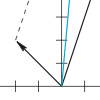
\includegraphics{1_1.jpg}

Portion of Fig. 2.2 from the textbook Introduction to Linear Algebra.
\end{center}

\noindent
The fundamental problem of linear algebra is to solve n linear equations in n unknowns; for example:
\[2x-y = 0\]
\[-x+2y = 3\]
The system above is two dimensional (n = 2). By adding a third variable z
we could expand it to three dimensions.

\noindent
In this first lecture on linear algebra we view this problem in three ways:

\begin{itemize}
\item Row Picture
\item Column Picture
\item Matrix Picture
\end{itemize}

\subsection*{Row Picture}

\noindent
Plot the points that satisfy each equation. The intersection of the plots (if they do intersect) represents the solution to the system of equations. Looking at Figure 1 we see that the solution to this system of equations is x = 1, y = 2.

\begin{center}
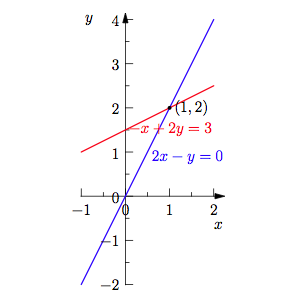
\includegraphics{Geometry1.png}

Figure 1: The lines 2x - y = 0 and -x + 2y = 3 intersect at the point (1, 2)
\end{center}

\noindent
We plug this solution in to the original system of equations to check our work:\\

\[2\cdot1-2 = 0\]
\[-1+2\cdot2 = 3\]

The solution to a three dimensional system of equations is the common point of intersection of three planes (if there is one).

\subsection*{Column Picture}

\noindent
In the column picture we rewrite the system of linear equations as a single equation by turning the coefficients in the columns of the system into vectors:\\

\[x\verticalvector{\phantom{-} 2\\-1} + y\verticalvector{-1\\\phantom{-} 2} = \verticalvector{0\\3}\]\\

Given two vectors c and d and scalars x and y, the sum xc + yd is called a linear combination of c and d. Linear combinations are important throughout this course.

\noindent
Geometrically, we want to find numbers x and y so that x copies of vector $\verticalvector{\phantom{-}2\\-1}$ added to y copies of vector $\verticalvector{-1\\\phantom{-}2}$ equals to vector $\verticalvector{0\\3}$. As we see from Figure 2, x = 1 and y = 2, agreeing with the row picture in Figure 2

\begin{center}
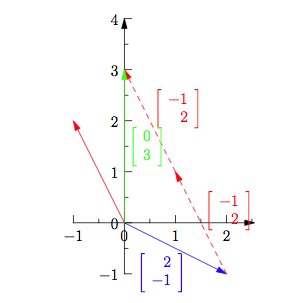
\includegraphics{Geometry2.png}

Figure 2: A linear combination of the column vectors equals the vector b.

\end{center}

\noindent
In three dimensions, the column picture requires us to find a linear combinations of three 3-dimensional vectors that equals the vector b.

\subsection*{Matrix Picture}


\noindent
We write the system of equations
\[2x-y = 0\]
\[-x+2y = 3\]
as a single equation by using matrices and vectors:

\[\begin{bmatrix} \phantom{-}2 & -1\\ -1 & \phantom{-}2 \end{bmatrix} \begin{bmatrix} x\\y \end{bmatrix} =  \begin{bmatrix} 0\\3 \end{bmatrix}\]\\

\noindent
The matrix $A = \begin{bmatrix} \phantom{-}2 & -1\\-1 & \phantom{-}2 \end{bmatrix}$ is called the coefficient matrix. The vector $x = \begin{bmatrix} x\\y \end{bmatrix}$ is the vector of unknowns. The values on the right hand side of the
equations form the vector \textbf{b}:

\[A\textbf{x} = \textbf{b}\].

\noindent
The three dimensional matrix picture is very like the two dimensional one, except that the vectors and matrices increase in size.
\par

\noindent
\textbf{Matrix Multiplication}\\
How do we multiply a matrix A by a vector x?\\

\[\begin{bmatrix} 2 & 5\\ 1 & 3 \end{bmatrix} \begin{bmatrix} 1\\2 \end{bmatrix} = ?\]\\

\noindent
One method is to think of the entries of x as the coefficients of a linear combination of the column vectors of the matrix:

\[\begin{bmatrix} 2 & 5\\ 1 & 3 \end{bmatrix} \begin{bmatrix} 1\\2 \end{bmatrix} = 1\begin{bmatrix} 2\\1 \end{bmatrix} + 2 \begin{bmatrix} 5\\3 \end{bmatrix} = \begin{bmatrix} 12\\7 \end{bmatrix}\]\\

\noindent
This technique shows that Ax is a linear combination of the columns of A. \par 
\noindent
You may also calculate the product Ax by taking the dot product of each row of A with the vector x:

\[\begin{bmatrix} 2 & 5\\ 1 & 3 \end{bmatrix} \begin{bmatrix} 1\\2 \end{bmatrix} = \begin{bmatrix} 2 \cdot 1 + 5 \cdot 2\\ 1 \cdot 1 + 3 \cdot 2 \end{bmatrix} = \begin{bmatrix} 12\\7 \end{bmatrix}\]

\noindent
\textbf{Linear Independence} \\

\noindent
In the column and matrix pictures, the right hand side of the equation is a vector b. Given a matrix A, can we solve:
\[Ax = b\]
\noindent
for every possible vector b? In other words, do the linear combinations of the column vectors fill the xy-plane (or space, in the three dimensional case)? \\

\noindent
If the answer is "no", we say that A is a singular matrix. In this singular case its column vectors are linearly dependent; all linear combinations of those vectors lie on a point or line (in two dimensions) or on a point, line or plane (in three dimensions). The combinations don't fill the whole space.

\end{document}
